\section{Runterschreiben}
\label{sec:rusch}



\subsection{Problem - \enquote{dürftiges} Bremsverhalten}

Die Simulationsplattform bietet durch realistisch modellierte Beschleunigungen und Verzögerungen den Vorteil, dass der Verkehr realistischer, feingranularer abgebildet werden kann.
Die analog zu den Simulationen von Nagel und Schreckenberg gewählte Zellgröße von $7,5$ Metern führt allerdings dazu, dass theoretisch dargestellte Reduktionen der Geschwindigkeit nicht direkt in nächsten Zeitschritt umgesetzt werden.
Vielmehr muss, wie auch beim losfahren, siehe \cref{sec:accelerategroove}, ein gewisser Wert unterschritten werden, damit die gezeigte Bewegung auch real kürzer gesetzt wird.

Dieses Verhalten kann durch Reduktion der Zellgröße 



\subsection{Problem - \enquote{Eingrooven} am Anfang der Simulation}
\label{sec:accelerategroove}

Aufgrund der vergleichbar zum NaSch-Modell gewählten Zellgröße von $7,5 m$, im Gegensatz dazu aber die Simulation realitätsnaher Beschleunigungswerte, kommt es zu Simulationsbeginn mehrere Zeitschritte lang zu einem Stillstand der Fahrzeuge.
Da jedes Fahrzeug softwareseitig in der Mitte der belegten Zelle platziert wird (bzw. im ersten Schritt dorthin \enquote{zurückrutscht}) wird eine Geschwindigkeit von mehr als $ \frac{1}{2} \times 7,5 \frac{m}{s} = 13,5 km/h$ benötigt, um eine sichtbare Bewegung durchzuführen.
Durch die unterschiedliche Ausprägung der Beschleunigungswerte ist keine Nennung eines festen Zeitpunkts möglich, an dem dies vollzogen wird.

Im weiteren Verlauf der Simulation fällt es nicht weiter auf, dass die Fahrzeuge an Zellen mit einer bestimmten Länge gebunden sind.



\subsection{Entwicklung/Entscheidung - Festlegen der Trödelparameter}

Im Originalmodell wird dem jeweiligen Fahrzeug im Trödelfall eine Geschwindigkeitseinheit wieder abgezogen. 
In jenem Zeitschritt erfolgt somit keine Beschleunigung, bzw. bei Fahren mit max. möglicher Geschwindigkeit wird diese reduziert. 
Auf das Abbremsen vor einem Hindernis hat dies keinen merklichen Einfluss, weil die Geschwindigkeit an Größe der Lücke angepasst wird.

Für die Simulation musste ein Wert gefunden werden, der dieses Verhalten annähernd trifft.
Im Laufe mehrerer Testdurchgänge schien eine Intensität der Verzögerung von $0,3$ die getätigte Beschleunigung am besten zu egalisieren. 
Hierbei ist noch die Streuung der Beschleunigungs- und Verzögerungswerte zu beachten, sodass das Trödeln unterschiedliche Effekte haben kann.

Für das Abbremsen in der Agentensimulation kann sich das Trödeln positiv auf den Bremsweg auswirken.



\subsection{Entwicklung/Entscheidung - Festlegen der view range}

Das originale Modell von Nagel und Schreckenberg legt Beschleunigung, Verzögerung und Sichtfeld sehr einfach fest.
Bedingt durch die Zellgröße von 7,5 m, die Ganzzahligkeit der Geschwindigkeit und die Zeitschrittlänge von 1 Sekunde ergeben sich Beschleunigungswerte von $7,5 \frac{m}{s^{2}}$. 
Durch die Möglichkeit, die Geschwindigkeit innerhalb eines einzigen Zeitschrittes von der Maximalgeschwindigkeit \enquote{5} auf Null zu verringern, ergibt sich theoretisch eine Verzögerung von $37,5 \frac{m}{s^{2}}$.

Die Simulationsumgebung arbeitet hier mit realen Werten zwischen $3,5$ und $7 \frac{m}{s^{2}}$ für die Beschleunigung und zwischen $8$ und $10 \frac{m}{s^{2}}$ für die Verzögerung.
Der Wert wird für jedes Fahrzeug bei der Initialisierung im Rahmen dieser Intervalle zufällig festgelegt.
Die Dosierung der möglichen Beschleunigung bzw. Verzögerung wird im Agent-Script festgelegt.

Für die Sichtweite ergibt sich für im NaSch-Modell der theoretische Wert von $5 \times 7,5 m$, also $37,5$ Meter.
Dies ist in dieser Simulation unmöglich.
Laut [Arbeit] liegt die Sichtweite auf Autobahnen zwischen $210$ und $360$ Metern.
Ein Wert von $250 m$ erscheint realistisch und sinnvoll und wurde gewählt.



\subsection{Problem - Sichtfeld der Fahrzeuge}

Um die Position eines anderen Fahrzeugs in der Umwelt festzustellen, kann die Richtung, in der dieses sich befindet, bestimmt werden.
Die Simulationsumgebung hatte für das Sichtfeld der Fahrzeuge eine Unterteilung in acht Sektoren vorgesehen, so dass neben den Richtungen vorwärts, rückwärts, links und rechts auch Unterscheidung in Zwischenschritte möglich war, siehe \cref{figure:car-view-sectors} (a).

\begin{figure}[hptb]
  \centering 
   \subfigure[acht Sektoren]{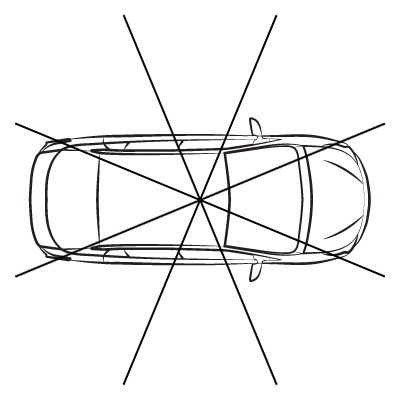
\includegraphics[width=0.3\textwidth]{car-view-8sectors}}\qquad 
   \subfigure[zwei Sektoren]{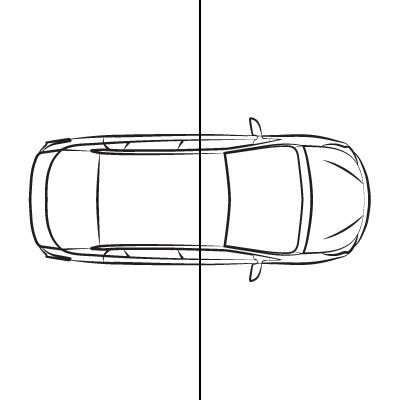
\includegraphics[width=0.3\textwidth]{car-view-2sectors}}\qquad 
   \subfigure[vier Sektoren]{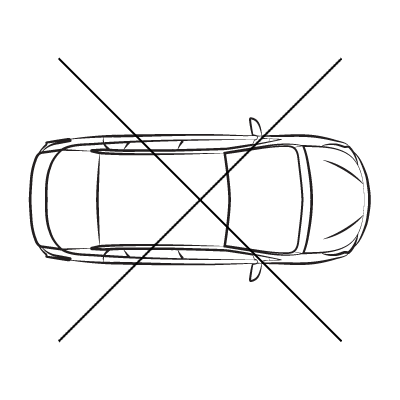
\includegraphics[width=0.3\textwidth]{car-view-4sectors}}
  \caption{mögliche Sichtfelder eines Fahrzeugs, Quelle: Auto-Silhouette vecteezy.com} 
  \label{figure:car-view-sectors}
\end{figure}

Eine solch feine Unterscheidung war nicht nötig.
Es sollte genügen, feststellen zu können, ob sich ein anderes Fahrzeug relativ zu \enquote{Ego} im vorwärtigen oder rückwärtigen Raum befindet. 
Die Abdeckung sollte ohne Unterbrechung sein.
Für die Simulation nach dem Einspurmodell von Nagel-Schreckenberg funktionierte dies ohne Probleme.
Bei einem Testlauf des Mehrspurmodells mit vier Fahrzeugen kam es zur Kollision zweier Fahrzeuge. 
Bei der anschließenden Kontrolle stellte sich heraus, dass ein Fahrzeug (vehicle0), welches sich auf der Überholspur (lane 2) befand, ein anderes Fahrzeug (vehicle20) direkt neben sich nicht \enquote*{sah} und daraufhin, so wie es der Plan vorsah, zum nächsten Schritt in die Hauptspur fährt. 
Im nachfolgenden Zeitschritt kam es dann zur Kollision.

\begin{verbatim}
--- step 365 ----------------
         vehicle20   in lane   1   in cell   333.0   @   74.21582362319865   kph
         vehicle2   in lane   1   in cell   282.0   @   129.99324819683062   kph
         vehicle0   in lane   2   in cell   333.0   @   99.94723620551235   kph
PIA1     vehicle0   sees no traffic at all -> Pull-in
         vehicle1   in lane   1   in cell   90.0   @   130.8321253026147   kph
--- step 366 ----------------
         vehicle20   in lane   1   in cell   4.0   @   74.21582362319865   kph
         vehicle2   in lane   1   in cell   289.0   @   131.11124225593747   kph
         vehicle0   in lane   1   in cell   3.0   @   100.80986539456516   kph
TFC100   vehicle0   has vehicle in-front of -> decelerate
COS      vehicle0   STOPPED -> collision
OUT      vehicle0   -> Pull-out attempt successful
         vehicle1   in lane   1   in cell   97.0   @   130.64144521630223   kph
\end{verbatim}

Das Sichtfeld der Fahrzeuge wurde zu einem Vier-Sektoren-Modell abgewandelt und die Pläne für Ein- und Ausscheren, der hiervon gleichermaßen betroffen sein dürfte, angepasst.
Es werden nun jeweils die beiden Sektoren, die die Bewegungs- bzw.Orientierungsrichtung darstellen, kontrolliert.